\documentclass[10pt,a4paper]{article}
\usepackage[utf8]{inputenc}
\usepackage[T1]{fontenc}
\usepackage{amsmath}
\usepackage{amssymb}
\usepackage{graphicx}
\usepackage{hyperref}
\usepackage{float}
\usepackage{subcaption}
\usepackage{geometry}
\geometry{a4paper, margin=1in}

\title{Exploring the Platonic Representation Hypothesis Beyond In-Distribution Data}
\author{Aryasomayajula Ram Bharadwaj\\
Independent Researcher\\
\texttt{ram.bharadwaj.arya@gmail.com}}
\date{20th Oct 2024}

\begin{document}

\maketitle

\begin{abstract}
The Platonic Representation Hypothesis (PRH) \cite{huh2024prh} posits that neural networks, despite being trained on different objectives and datasets, converge toward a shared statistical model of reality. This paper extends the investigation of PRH to out-of-distribution (OOD) settings, using ImageNet-O as a benchmark, and contrasts the findings with results from in-distribution data and random noise. Our analysis reveals that while PRH holds in OOD scenarios, it breaks down with purely random data, suggesting that a common underlying structure in the data is essential for representational alignment.
\end{abstract}

\section{Introduction}
The PRH suggests that models trained across various modalities and objectives converge toward a shared representation of reality \cite{huh2024prh}. Inspired by philosophical concepts like Plato’s Allegory of the Cave, PRH proposes that neural networks are progressively learning an idealized representation of the world. This convergence has been observed across domains such as vision and language models, with evidence showing that larger models better align their internal representations \cite{huh2024prh}. However, it remains unclear whether such convergence persists when models encounter data significantly different from their training distribution.

To address this, we extend PRH's analysis to out-of-distribution (OOD) settings using the ImageNet-O dataset, which contains samples outside the distribution of ImageNet \cite{hendrycks2021nae}. We also include random noise as a contrasting dataset to examine the boundaries of representational alignment.

\section{Methodology}
We assess representational alignment using various metrics, such as mutual k-NN and CKNN-A, across three types of data:
\begin{enumerate}
    \item \textbf{In-distribution data}: Data that aligns with the pretraining dataset (e.g., Places365’s validation set).
    \item \textbf{Out-of-distribution data}: ImageNet-O, designed with images that are outliers to the ImageNet distribution \cite{hendrycks2021nae}.
    \item \textbf{Random noise}: Purely random images to test the limits of PRH.
\end{enumerate}
The alignment between different models is measured using Spearman's rank correlation, focusing on how similar the models' distance measures are for given data points.

\section{Results}

\subsection{Vision-Vision Alignment on In-Distribution Data}
\begin{figure}[H]
    \centering
    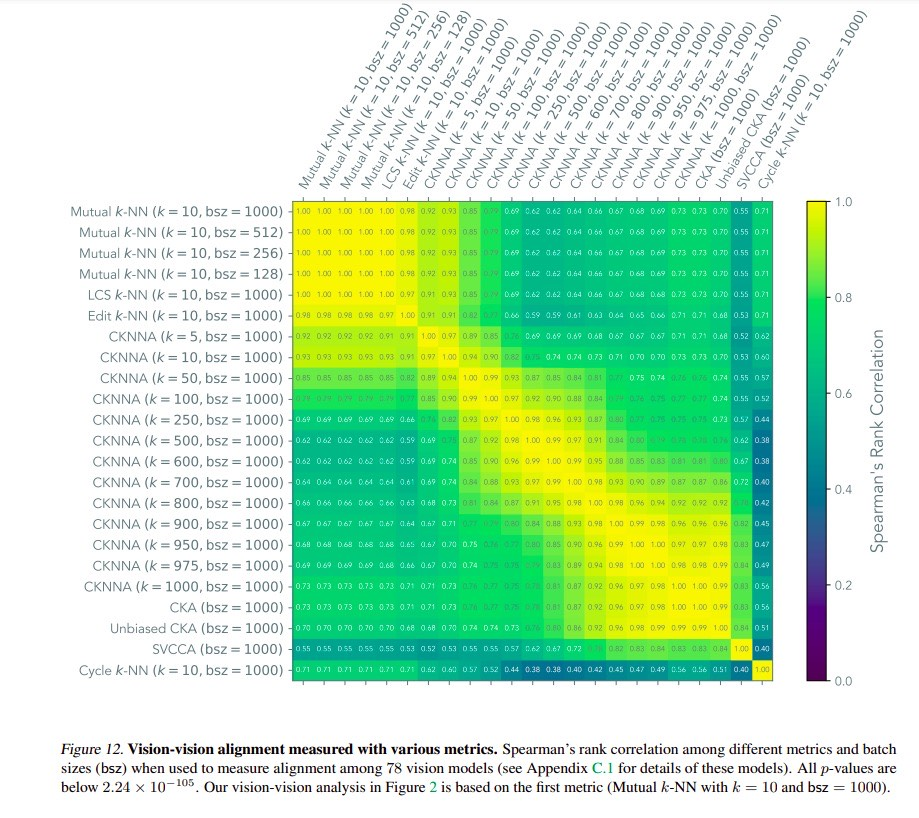
\includegraphics[width=\textwidth]{prh_correlation.jpg}
    \caption{Vision-vision alignment measured on Places365’s validation dataset using various metrics. High Spearman's rank correlation among different metrics indicates alignment among vision models.}
    \label{fig:prh_correlation}
\end{figure}

\subsection{Vision-Vision Alignment on ImageNet-O}
\begin{figure}[H]
    \centering
    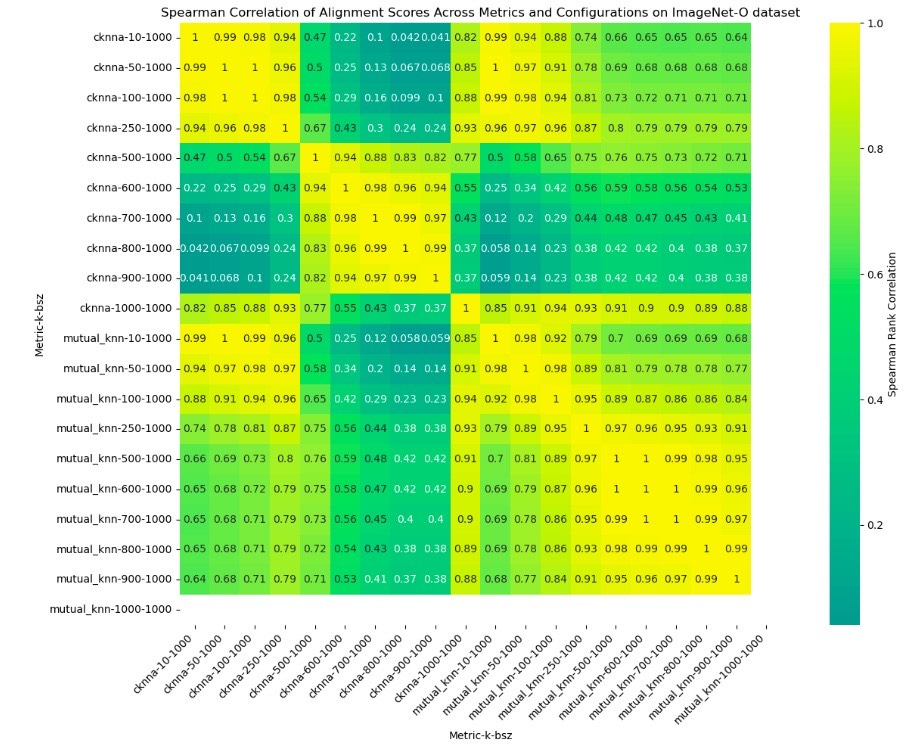
\includegraphics[width=\textwidth]{prh_correlation_ood.jpg}
    \caption{Alignment of models on ImageNet-O dataset. The Spearman correlation suggests that even with outlier data, models maintain a shared statistical representation, albeit with higher prediction errors.}
    \label{fig:prh_correlation_ood}
\end{figure}

\subsection{Vision-Vision Alignment on Random Data}
\begin{figure}[H]
    \centering
    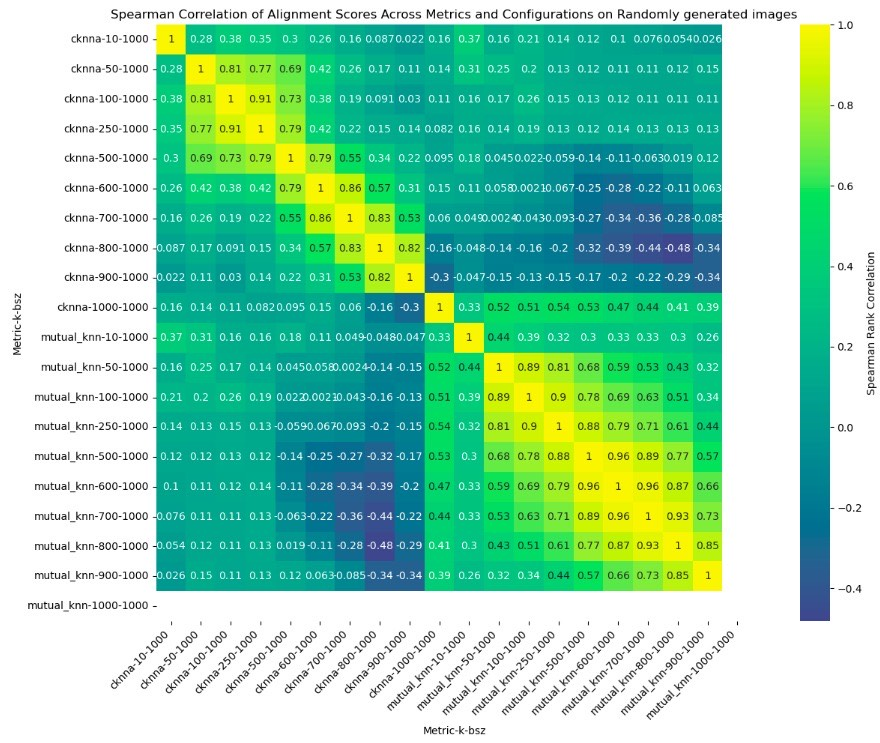
\includegraphics[width=\textwidth]{prh_correlation_random.jpg}
    \caption{Spearman correlation of alignment scores on random noise data. The lower correlation values indicate a breakdown in representational alignment, suggesting that random data lacks the underlying structure needed for PRH.}
    \label{fig:prh_correlation_random}
\end{figure}

\section{Discussion}
Our findings show that PRH extends beyond in-distribution data to OOD settings, where models exhibit alignment in their internal representations. On ImageNet-O, models align in their predictions even when they produce incorrect results with high confidence, revealing that models fail in a predictable manner on OOD data. This suggests that they rely on a shared interpretation of the input space, even when the data diverges from what they have seen during training.

However, this alignment does not extend to purely random data, where the lack of structure prevents models from developing a shared statistical understanding. This distinction emphasizes that the presence of meaningful underlying structure is a prerequisite for representational convergence, aligning with PRH's notion of a shared representation of reality.

\section{Conclusion}
The results validate the Platonic Representation Hypothesis in OOD scenarios but highlight its limitations with random noise. Our analysis underscores the need for structured data in achieving representational alignment and suggests new directions for exploring the boundaries of PRH. Future work could focus on extending PRH to other modalities and finding conditions where the hypothesis might be challenged or refuted.

\vfill
The code used for the experiments and analysis in this paper is available on GitHub at \href{https://github.com/rokosbasilisk/prh-experiments}{https://github.com/rokosbasilisk/prh-experiments}.

\clearpage
\begin{thebibliography}{9}

\bibitem{huh2024prh}
Huh, M., Cheung, B., Wang, T., \& Isola, P. (2024). The Platonic Representation Hypothesis. \emph{International Conference on Machine Learning}.

\bibitem{hendrycks2021nae}
Hendrycks, D., Zhao, K., Basart, S., Steinhardt, J., \& Song, D. (2021). Natural Adversarial Examples. \emph{CVPR}. \href{https://arxiv.org/abs/2405.07987}{arXiv:2405.07987}.

\end{thebibliography}

\end{document}

